\chapter{GPU Based Algorithms for Spectrum Sensing in Cognitive Radio Networks}
\label{chap:cognet_gpu}
\section{Introduction}
The idea of opportunistic spectrum sharing has seen heavy focus in the cognitive radio research community.  The use of efficient spectrum sensing algorithms is necessary to facilitate this.  As such, much of the research has focused on the development of these efficient spectrum sensing algorithms.  Various methods have been proposed such as energy detection \cite{CabTkaBro06}\cite{HurParWoo06}, cyclostationary spectral analysis \cite{FenBos07}\cite{OshClaEbe07}, and collaborative based approaches \cite{GanLi05}\cite{SadAzm08}.  Overall the computational performance of these algorithms requires improvement in order to be truly viable in order to perform real time spectrum sensing.

The goal of our work here is to implement well defined methods of spectrum sensing on a new computing architecture, a programming Graphics Processing Unit (GPU).  We show that this computing architecture greatly improves the performance of these spectrum sensing algorithms both in terms of run times as well as amount of complex computational work they can achieve in a reasonable time.  In Section~\ref{sect:gpu_related_work} we discuss some of the related work around improving the performance of spectrum sensing algorithms.  

This chapter is organized as follows: Section~\ref{sect:gpu_why_use_gpu} discusses why the GPU is a viable computing architecture for improving the performance of spectrum sensing algorithms.  Section~\ref{sect:gpu_spect_sensing_algos} then presents the algorithms we consider for implementation on the GPU.  In Sections \ref{sect:gpu_experiment} and \ref{sect:gpu_results} we present the testing environment, test data used, and the results we gathered from the comparison of running these algorithms on the CPU vs the GPU.  Sections \ref{sect:gpu_conclusion} and \ref{sect:gpu_future_work} then closes with our conclusions on our findings and a short discussion of our future work.

\section{Related Work}
\label{sect:gpu_related_work}
The literature surrounding the topic of spectrum sensing in cognitive networks is very broad.  Several different works have focused on means of improving the performance of existing spectrum sensing algorithms.  The work done in \cite{HurParWoo06} and \cite{QuaCuiSay08} focus on algorithms for wide-band spectrum sensing.  These algorithms focus on detecting spectral holes in multiple sub-channels in a single pass of an algorithm rather than searching for spectral holes one sub-channel at a time.

Further work has focused on the development of co-operative spectrum sensing techniques, such as the work done in \cite{GanLi05} and \cite{SadAzm08}.  Co-operative based spectrum sensing aims to improve the performance and reliability of spectrum detection by having multiple nodes in the network work together in detecting spectral holes.  These methods have been shown to improve performance but have not considered the possibility of using a different computing architecture to further improve performance.

The work done in \cite{OshClaEbe07} and \cite{FenBos07} have aimed to improve the overall performance of their spectrum sensing algorithms by porting them onto the IBM Cell processor in a Playstation 3.  The architecture of the Cell processor is one meant for highly efficient parallel computation, which provided great benefit to the spectrum sensing algorithms used in the aforementioned works.  In \cite{FenBos07} they say that the performance increase they got was limited by two factors.  First the latency of transferring the data from its source to the Cell processor was significant which hurts potential real time performance.  The second limiting factor was the data rate limits of USB2, which was used in transferring the signal data from its source to the Cell processor in the Playstation 3, limited the signal bandwidth they could work with.

Overall the literature has shown many ways in which to increase the performance of spectrum sensing algorithms.  Yet no one has yet made an attempt to port these algorithms onto a General Purpose Graphics Processing Unit (GPGPU).  The novelty of our work here is showing how several of these algorithms can be ported to the GPU, and to show the performance gains achieved by doing so.

\section{Why Use the GPU?}
\label{sect:gpu_why_use_gpu}
The GPU is a highly parallelized, multi-threaded, multi-cored processor.  The GPU is well suited to address problems that can be expressed as data-parallel computations - the same program executing on many data elements in parallel - with high arithmetic intensity \cite{Nvidia08}.  A single GPU is capable of computing thousands of threads simultaneously with incredibly optimized performance for high precision floating point operations.  Figure \ref{fig:cpu_vs_gpu_arch} illustrates the difference in architecture between CPUs and GPUs.  Since GPUs are specialized for data parallelism, they have a lower requirement for flow control and memory access latency can be hidden with high intensity calculations instead of data caches \cite{Nvidia08}.  

%should use some of the diagrams from the Nvidia CUDA Programming Guide
\begin{figure}[ht]
\begin{center}
 \scalebox
 {0.80} % h_length
 {
 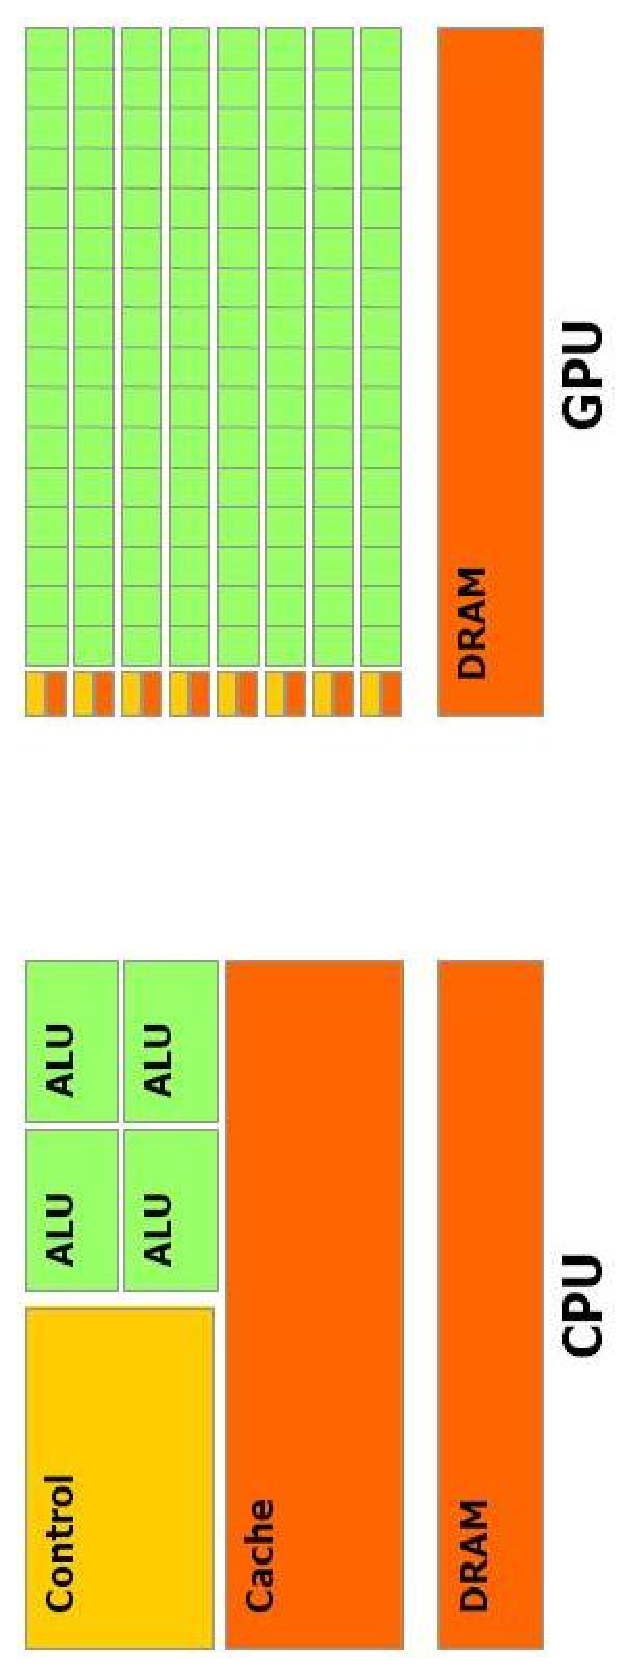
\includegraphics[angle=270,scale=0.5]{images/gpu_images/cpu_vs_gpu_arch.eps}
 }
\end{center}
\caption{Basic diagrams comparing the differences in the architectures between a CPU and a GPU.  The GPU clearly devotes more transistors to data processing \cite{Nvidia08}.}
\label{fig:cpu_vs_gpu_arch}
\end{figure}

Ultimately this difference in architecture translates to higher throughput of floating point operations per second.  Figure \ref{fig:cpu_vs_gpu_gflops} shows a comparison of different GPU cores vs different CPU cores over a given time line.  The comparison shows the growth in peak performance measured in GFLOPS.  We can clearly see that GPU's peak performance has grown significantly higher than that of any CPU currently on the market.  This makes the GPU seem like the ideal platform on which to perform large scale complex computations.

\begin{figure}[ht]
\begin{center}
 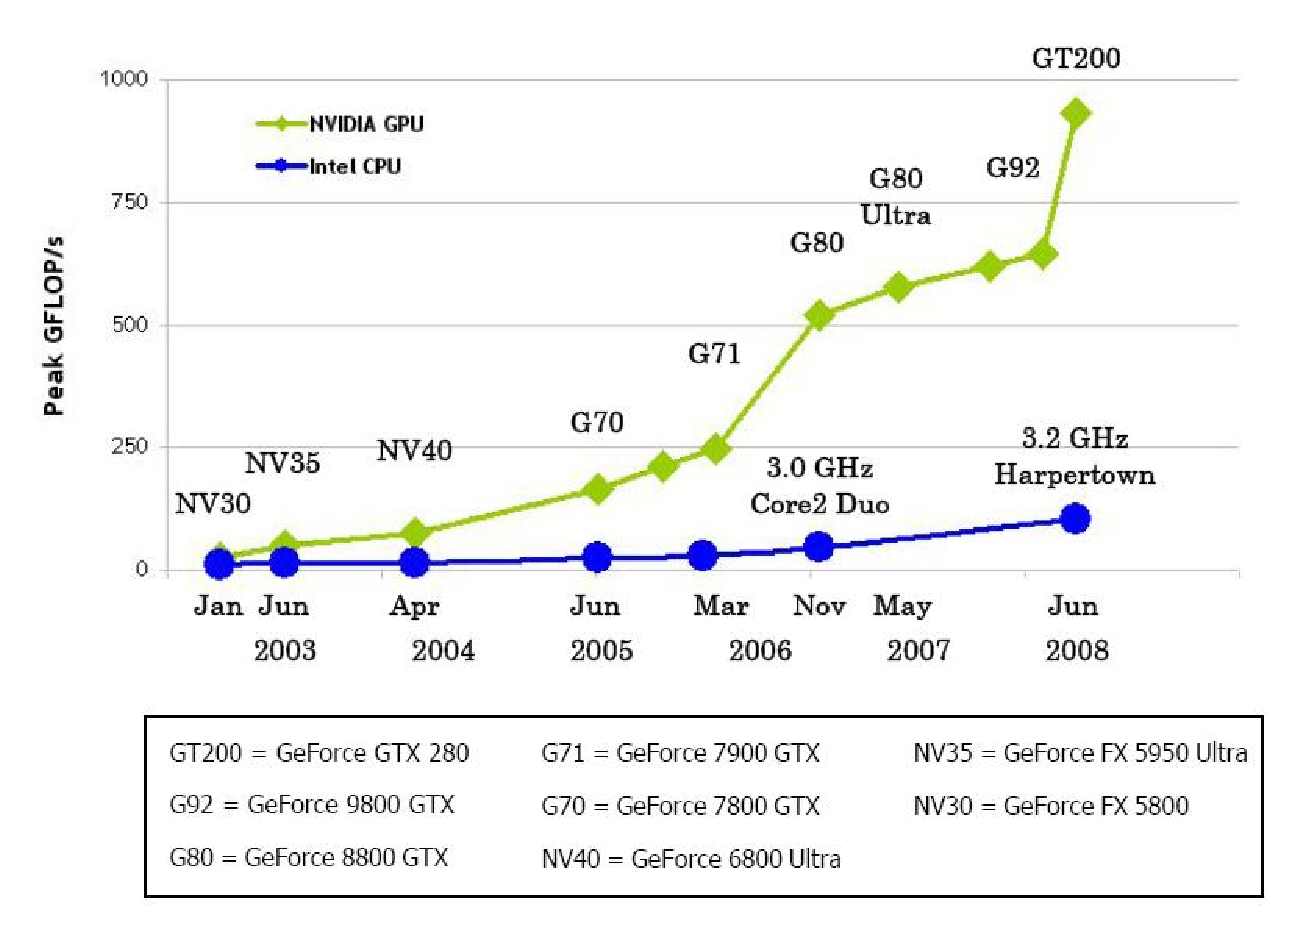
\includegraphics[scale=0.65]{images/gpu_images/cpu_vs_gpu_gflops.eps}
\end{center}
\caption{Graph showing a comparison of growth in peak performance between GPU's and CPU's over a given time line \cite{Nvidia08}.}
\label{fig:cpu_vs_gpu_gflops}
\end{figure}

%Not sure this fits in this section or maybe just this location, see if it can be moved or needs to be removed.
Through NVIDIA's CUDA computing engine, the massively parallel structure of GPU's can be harnessed for general purpose computing.  CUDA provides extensions to industry standard languages, such as C and Python, to access the parallel computing capabilities of NVIDIA based GPU's.  CUDA provides a set of three key abstractions - a hierarchy of thread groups, shared memory, and barrier synchronization - that are exposed to the programmer through these language extensions \cite{Nvidia08}.

\subsection{Application to Cognitive Networking}
\label{subsect:app_to_cognet}
Cognitive networking algorithms rely on extremely fast computations of large sets of complex data in order to provide the necessary real time requirements for performance.  In many cases, these computations can take advantage of parallel computing architectures, such as those offered by GPUs, to help increase their performance.

One of the primary operations relied upon by many of the cognitive networking algorithms is the computation of Fast Fourier Transformations (FFT)  This is a common operation in many signal processing algorithms and is one that can benefit from a high degrees of parallelism.  Algorithms such as the FFT Accumulation Method (\ref{sect:FAM}) make heavy use of FFTs, so a fast implementation can make a big difference in the algorithms overall performance.  Figure \ref{fig:matlab_vs_gpu_fft_timings} shows a comparison of computation times for FFTs of complex signals of varying size using Matlab and using CUDA for GPU execution.  The CUDA computations times include the necessary time to transfer the signal data from host memory (RAM) into device memory (GPU RAM).  Please see section \ref{sect:test_platform} for details on the testing platform used to generate these results.

\begin{figure}[ht]
\begin{center}
 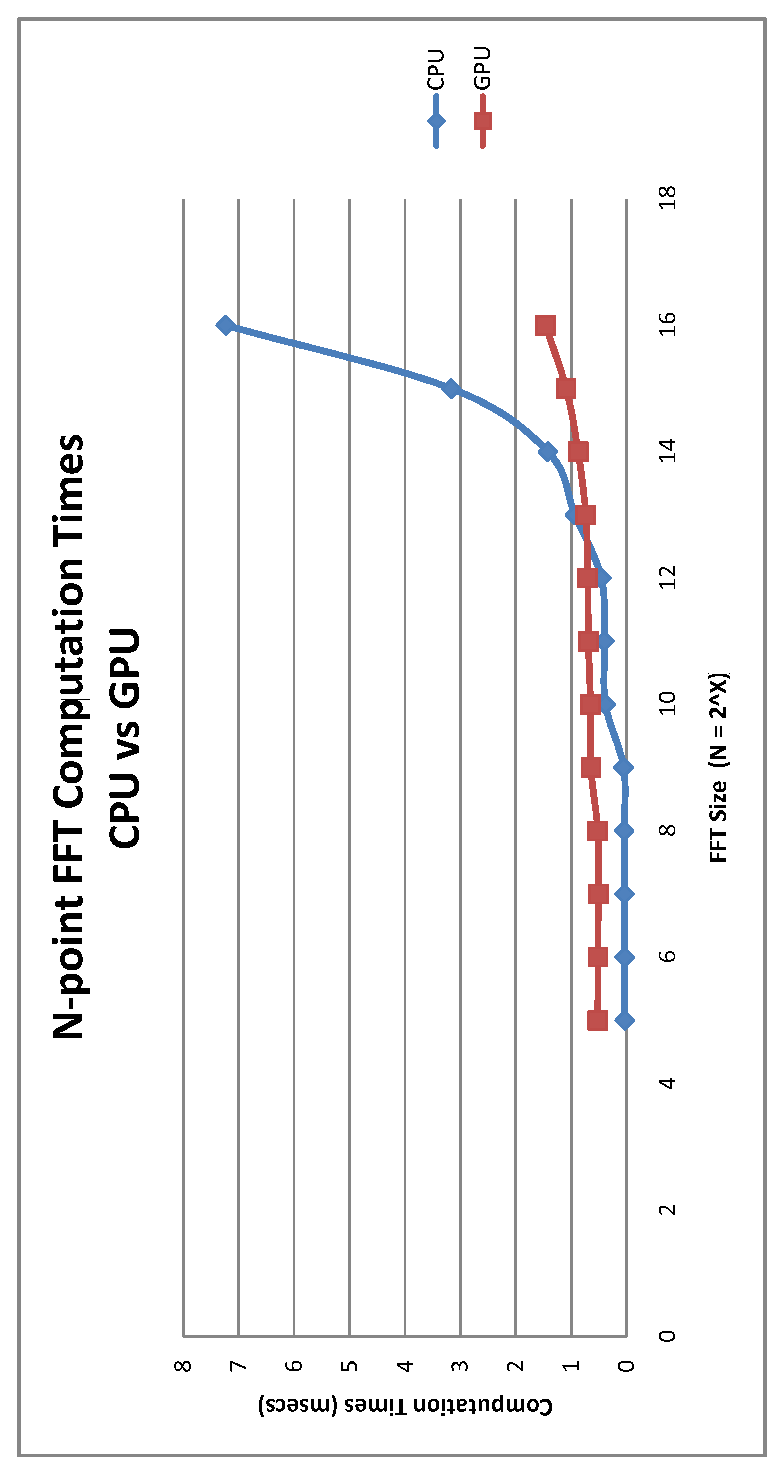
\includegraphics[angle=270,scale=0.6]{images/gpu_images/matlab_vs_cuda_fft_timings.eps}
\end{center}
\caption{Graph showing a comparison of computations times for FFTs of varying sizes in Matlab and on a GPU.}
\label{fig:matlab_vs_gpu_fft_timings}
\end{figure}

In analyzing this graph we can see as the size of the FFT increases, Matlab hits a point where computations times grow exponentially while computations on the GPU continue to grow in a slow linear fashion.  This crossover point occurs at sizes of $N = 2^13 = 8192$ and greater.  Signal data containing this many discrete points is not out of the question, especially when performing wide-band spectrum sensing.  

At the same time this graph exposes a weakness of computing on the GPU.  At sizes below the switching threshold, the GPU's performance has a floor which is does not go below.  This is because of the overhead associated with a) transferring the data from host memory to device memory, b) setting up the necessary framework for parallel computation.  Regardless of the amount of data being processed these factors are always present. Therefore to negate the computational overhead gained from these factors the GPU should be saturated with as much data as possible and perform computations of a complex enough nature in order to see the most benefit from its massively parallel architecture.  At sizes below $N = 8192$ the GPU was simply not receiving enough data to negate the computational overhead of performing a single FFT.

This is a fairly simplified example since we are only computing a single FFT.  Typical algorithms will require much more complex computation than just a single FFT so the mentioned overhead associated with GPU computations will usually be easily negated.  As such these signal size thresholds do not hold as concrete threshold values to be targeted when considering the GPU for computing an algorithm.

Despite this weakness if using the GPU for computations, as mentioned previously, the need to process large amounts of signal data is not uncommon.  Therefore when performing more wide-band operations, the GPU will likely still have a strong upper hand over traditional CPU computations.

\subsection{Availability and Cost Effectiveness}
The GPU is also a very cost effective and readily available solution.  Almost every desktop, and even some laptop computers, sold today have some version of a GPU residing in them.  Even those desktop computers without a GPU can easily add them one to its setup, and at a fairly reasonable price too.  

Although cell processors are also very powerful and highly parallelizable, they are not yet as widely available as GPU's in everyday computing devices.  The only commercially available device with a cell processor is the Sony Playstation 3.  It is possible to use the cell processor in the Playstation 3 for general purpose computing, as evidenced by the work done in \cite{FenBos07}, but it requires the purchase and presence of the entire Playstation 3 hardware setup.  It may not be feasible or desirable to have an extra hardware piece such as the Playstation 3 tied to a real world cognitive radio.  As described by \cite{FenBos07} there is also significant latency associated with transferring the necessary data from its source to the Playstation 3 for processing.  This is due in part to the lack of a capable high speed bus through which to transfer data into the Playstation 3.  GPU's do not suffer from problem as they have a dedicated high speed bus connection through a computers motherboard.  From both a cost and availability standpoint, GPU's are an excellent choice for adapting cognitive networking algorithms.


\section{Spectrum Sensing Algorithms}
\label{sect:gpu_spect_sensing_algos}
The cognitive networking model assumes two kinds of users, primary and secondary users.  Primary users are those who have privileged rights to a licensed spectrum for their commercial or public usage.  Secondary users are those users who do not have privileged rights but still have access to licensed spectrums.  These secondary users must opportunistically use unallocated spectrum resources when they are available, but vacate those resources when a primary user desires access to them.  In order to facilitate the intelligent usage of unallocated resources, secondary users must have a means of detecting the unused portions of a spectrum.  Spectrum sensing algorithms are designed to quickly and accurately detect the unoccupied spectrum segments available for use by secondary users.

There are several methods available to perform this kind of detection.  Each method is suited to different types of environments and signal types.  We have chosen to target two methods for this paper, energy detection and cyclostationary spectral analysis.

\subsection{Energy Detection}
\label{sect:energy_detect}
One of the potential methods available to perform spectrum sensing is through the use of an energy detector.  Energy detection is typically used to detect a weak deterministic signal in additive noise, which is assumed to be additive, white, and Gaussian \cite{CabTkaBro06}.  The energy detector works by measuring the energy in the received waveform over an observation time window \cite{CabTkaBro06}.

Energy detectors by nature have to be suboptimal.  This is due to the fact that in order to be optimal the detector would need to be based on a matched filter, thus requiring \textit{a priori} knowledge of the data for coherent processing \cite{CabTkaBro06}.  Knowing this, there are two possible ways of computing our suboptimal energy detector.  The first method uses a conventional energy detector which consists of the following parts: a low pass filter, a Nyquist sampling A/D converter, and a square-law device and integrator \cite{CabTkaBro06}.  Figure \subref{fig:energy_detect_a} provides a block diagram of this method.  The second method is devised through the use of a periodogram to estimate the spectrum via the squared magnitude of the FFT of the signal \cite{CabTkaBro06}.  Figure \subref{fig:energy_detect_b} illustrates a block diagram for this method.

\begin{figure} [ht]
%\begin{center}
\centering
	\subfigure[]{
		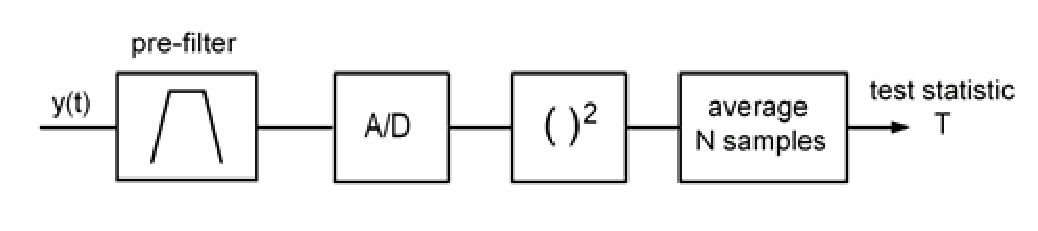
\includegraphics[scale=0.45]{images/gpu_images/energy_detector_a.eps}
		\label{fig:energy_detect_a}
	}
	\subfigure[]{
		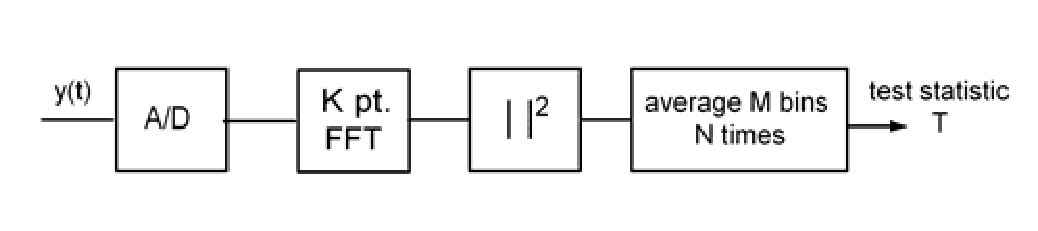
\includegraphics[scale=0.45]{images/gpu_images/energy_detector_b.eps}
		\label{fig:energy_detect_b}
	}
%\end{center}
\caption{Two possible implementations of an energy detector.  \subref{fig:energy_detect_a} uses an analog pre-filter and square-law device.  \subref{fig:energy_detect_b} uses periodogram: FFT magnitude squared and averaging. Image sourced from \cite{CabTkaBro06}}
\label{fig:energy_detect}
\end{figure}

For our work we have chosen to work with the periodogram based energy detector described by \cite{CabTkaBro06}.  Specifically, we have chosen the Welch method or averaged periodograms for estimating the Power Spectral Density (PSD) function as detailed in \cite{Welch67}.  This method breaks the signal data down into equal sized segments.  Each segment is defined to be of length $M$ and we can define segments to have an overlap of $D$ samples.  Each segment is then windowed, typically with a Hamming window.  Following this, a modified periodogram of each segment is calculated.  The computation of the modified periodogram consists of 1) taking the FFT of the segment data.  2) Finding the absolute value or magnitude of each sample and squaring it.  3) Each sample is then scaled by the value $\frac{1}{M}$.  Once the modified periodogram of each segment has been computed, all the segments are averaged together to form the PSD estimate.
The overlapping of the segments provides a decreased error variance in the final spectral estimate \cite{Welch67}.  It also has an effect on the number of segments available for averaging.  Greater overlap between segments means that more segments are able to fit within the same fixed signal size.  Changing of the parameter $M$ also effects the error variance by increasing or decreasing the number of averages we take to generate the final spectral estimate \cite{Welch67}.  As stated by \cite{CabTkaBro06}, the adjustment of the segment size $M$ also has an effect on the detectors performance.

\subsection{Cyclostationary Spectral Analysis}
\label{sect:cyclo}
Another method of performing spectrum sensing is through the use of cyclostationary spectral analysis.  This method is typically chosen to detect low SNR modulated signals because of its ability to distinguish between modulated signals, interference, and noise in low signal to noise ratios \cite{FenChenWan08}.  Cyclic spectral analysis algorithms work by estimating the correlation between spectral components of signals.  Spectral components are the complex envelopes of narrow-band, bandpass components of a signal \cite{RobBroLoo91}.  This correlation is described by the spectral correlation density (SCD) function.  This function describes the localization in the frequency domain of the amount of time-correlation between frequency-shifted versions of a given signal $x(t)$ \cite{Costa96}.  The SCD is represented by the two dimensional cyclic frequency and signal frequency space \cite{FenChenWan08} called the bi-frequency plane.  Presence of a signal can then be detected through the use of the SCD function \cite{Costa96}.

For our work we have chosen to implement the well known FFT Accumulation Method (FAM) to estimate the SCD function.  The FAM algorithms is of specific interest for adaptation onto a GPU because it is able to take great advantage of data-parallelism.  The following section gives details about the FAM algorithm

\subsubsection{FFT Accumulation Method}
\label{sect:FAM}
The FFT Accumulation Method works by dividing the bi-frequency plane into smaller regions called channel pair regions and computes the estimates one block at a time using FFTs \cite{Pace03}.  The values of the SCD function are described by equation \ref{eq:SCD}.

\begin{equation}
S^{\alpha}_{X_{N^\prime}} {(n L, f)}_{\Delta t} = \sum_{r=0}^{P-1} X_{N^\prime}(r L,f + \frac{\alpha}{2}) X_{N^\prime}^*(r L, f - \frac{\alpha}{2})
\label{eq:SCD}
\end{equation}

Equation \ref{eq:ComplexDemod} describes the computation of the channel pair regions, also called the complex demodulates.

\begin{equation}
X_{N^\prime}(n,f) = \sum_{n=0}^{N^\prime - 1} w(n) x(n) e^{-(i 2 \pi f n)/N^\prime}
\label{eq:ComplexDemod}
\end{equation}

Here \begin{math}w(n)\end{math} is a data tapering window (e.g., Hamming window), L is a decimation factor in the frequency domain \cite{FenChenWan08}, P is equal to \begin{math}N / L \end{math} where $N$ is the total number of samples in the signal and $N^\prime$ is equal to the number of samples in each complex demodulate.  In choosing the value of \begin{math}N^\prime \end{math} we must consider that the time-frequency resolution product \begin{math}N/N^\prime\end{math} must satisfy the condition \begin{math}N/N^\prime >> 1\end{math} in order to have a statistically reliable measurement \cite{RobBroLoo91}.  The value of $L$ is typically chosen to be \begin{math}L \le N^\prime / 4\end{math} in order to provide a good compromise between computational efficiency and minimizing cycle leakage and aliasing \cite{RobBroLoo91}.

The algorithm then occurs in three steps.  First the channelization of the input signal is performed by an $N^\prime$-point FFT being hopped over the signal data in blocks of $L$ samples.  The results from the FFT are then frequency shifted to baseband.  This produces the decimated complex demodulates \cite{RobBroLoo91}.  Second the product sequences are computed.  These are computed by multiplying each complex demodulate by the complex conjugate of each of the others \cite{Costa96}.  Once these are computed a $P$-point FFT is applied to each product sequence value.  The final step is to reorder the data from the product sequence such that it is ordered by cycle frequency vs frequency.

%Maybe break this section off into a section below on the GPU's applicability to cognitive networking.
The parallelism of this algorithm is a direct result of the independence of the product sequences both before and after their computation \cite{RobBroLoo91}.  This means that at each step of the algorithm, we can take advantage of high degrees of data-parallelism.  In step one, each complex demodulate can be independently computed.  The same can be said of computing the product sequences and applying the $P$-point FFTs to each of the product sequences.  This very high level of data-parallelism combined with the large amount of computation necessary makes this algorithm a strong candidate for GPU based processing.


\section{Experimental Setup}
\label{sect:gpu_experiment}
All of the algorithms were coded, compiled and tested on the platform detailed in Section \ref{sect:test_platform}.  Timings for GPU executions were taken using CUDA supplied timing methods called from within the CUDA code.  Timings in Matlab were done using the \textit{tic} and \textit{toc} function calls native to Matlab.

\subsection{Test Platform}
\label{sect:test_platform}
The primary testing platform used was a desktop computer with the following specifications:
\begin{itemize}
\item \textbf{CPU:} Intel Core 2 Duo E7200
	\begin{itemize}
	\item CPU Speed: 2.53 GHz
	\item Bus Speed: 1066 MHz
	\item L1 Data Cache Size: 32KB x 2
	\item L1 Inst. Cache Size: 32KB x 2
	\item L2 Cache Size: 3MB
	\end{itemize}
\item \textbf{RAM:} 4GB DDR2 800 Dual Channel
\item \textbf{Video Card:} Nvidia GeForce 9600 GT
	\begin{itemize}
	\item Memory: 512MB 256-bit GDDR3
	\item Memory Clock: 1900MHz
	\item Clock Speed: 700 MHz
	\item Stream Processors: 64
	\end{itemize}
\item \textbf{Operating System:} Microsoft Windows XP with SP 3
\end{itemize}

All GPU development was done using NVidia CUDA SDK version 2.1.  The C++ compiler used was from Microsoft Visual Studio 2005 Professional Edition.  All Matlab code was run using Matlab R2008a version 7.6.0.324.  Matlab did have its multi-threading options enabled.  This allows Matlab to automatically multi-thread some of its built in computations such as simultaneous computation of multiple FFTs and matrix multiplication.  No explicit multi-threaded programming was done within the Matlab code due to the lack of the Matlab Parallel Computing Toolbox.
%find the name of the matlab multi-threading toolbox.

\subsection{Test Data}
In testing the implementation of each of our algorithms we used a fixed set of data that we have collected.  The data we use is synthetic data generated by Matlab consisting of a sinusoid plus Additive White Gaussian Noise (AWGN), sampled at 40MHz.  We generated several different complex exponential signals with the sinusoid embedded at different frequencies.  We generated the following signals, a sinusoid at 1MHz, sinusoid at 2MHz, and one with 3 sinusoids, one at 650KHz, one at 1MHz, and one at 3MHz.  The discrete size of each signal was 16384 samples.

To make the data more realistic, it was also transmitted and received by a pair of WARP hardware nodes.  WARP stands for Wireless Open-Access Research Platform, which has been developed by Rice University.  This platform allow for the prototyping of advanced wireless networks.  For our sample data the signals were transmitted between two WARP nodes at 2.4 GHz.  During the transmission and receiving process, channel information was added into the signals, they were up converted and down converted, and some gain control was applied as well.  This did have the effect of adding in some extra noise to the signals.

This test data was first used to verify the correctness of our algorithms implementations in CUDA.  This data was evaluated by known working implementations of each algorithm.  Results from our implementations were then carefully compared against these results to verify correctness.  The data was then also used when generating the various timings for both our Matlab and CUDA based code.  This step was done after correctness had been verified.

\section{Results}
\label{sect:gpu_results}
This section outlines our experimental findings on the timing differences between standard CPU based implementations in Matlab versus the same implementation done on the GPU using NVidia CUDA.

\subsection{Energy Detection}
\label{sect:energy_detect_result}
As discussed in Section~\ref{sect:energy_detect}, we have chosen the Welch method based energy detector.  We have implemented this in both Matlab and on the GPU.  The following sections provide details on the implementation in Matlab and CUDA.  A discussion on the results found follows.

\subsubsection{Implementation}
The implementation of our energy detector is rather simple.  The Welch method is provided in Matlab as a built in function called \textit{pwelch}.  Our CUDA implementation of the Welch method follows the layout of the algorithm detailed in \cite{Welch67}.  The implementation has been optimized to run efficiently on the GPU.
\subsubsection{CPU vs GPU Timings}
The timing results from the Welch method based periodogram energy detector showed some very interesting, although not unexpected results.  Tables~\ref{tbl:pwelch_matlab_timings} and \ref{tbl:pwelch_cuda_timings} show these results.  As mentioned in Section~\ref{sect:energy_detect} varying the number of averages can improve the spectral estimate that is computed.  In the following tables, $M$ is the length of each segment of the signal, which is the number of points averaged to produce the result.  We also include timings of different percentages of overlay between segments to observe their effect on performance.

In looking at the Matlab timings we can see that as the segment size grows, the time for computation is reduced.  This is not surprising since larger segments means fewer segments to compute, thus reducing the volume of computations necessary.  We also observe that as the overlay increases the computation times rise for all segment sizes.  Again this is expected since more overlay allows for more segments to be produced, thus increasing the volume of calculations necessary to form the final estimate.  In each case we can see that increasing the overlay percentage from 25\% to 75\% at least doubles the computation time required.
 
\begin{table*}
\begin{center}
\begin{tabular}{|l|l|l|l|l|}
\hline
 & \multicolumn{4}{|c|}{Matlab} \\
\hline
M & 512 & 1024 & 2048 & 4096 \\
\hline
25\% Overlap & 15.987ms & 10.196ms & 11.523ms & 8.656ms \\
50\% Overlap & 22.818ms & 14.170ms & 26.370ms & 10.817ms \\
75\% Overlap & 42.717ms & 25.284ms & 26.428ms & 17.409ms \\
\hline
\end{tabular}
\caption{Timing results from Matlab execution of Welch's Method of averaged periodograms for estimation of PSD.  Timings showed for varying segment and overlap sizes.}
\label{tbl:pwelch_matlab_timings}
\end{center}
\end{table*}

Turning to the CUDA timings we see a much different story.  Unlike the Matlab timings, Table~\ref{tbl:pwelch_cuda_timings} shows very consistent timings across all variations of both segment size and overlay percentage.  We only observe a slight increase in computation time, between $0.2$ and $0.3$ milliseconds, as the segment size increases.  This minimal increase in computation times is negligible when compared to the fluctuation of times from Matlab.

\begin{table*}
\begin{center}
\begin{tabular}{|l|l|l|l|l|}
\hline
 & \multicolumn{4}{|c|}{CUDA} \\
\hline
M & 512 & 1024 & 2048 & 4096 \\
\hline
25\% Overlap & 1.490ms & 1.494ms & 1.543ms & 1.690ms \\
50\% Overlap & 1.465ms & 1.459ms & 1.572ms & 1.693ms \\
75\% Overlap & 1.457ms & 1.462ms & 1.555ms & 1.720ms \\
\hline
\end{tabular}
\caption{Timing results from CUDA execution of Welch's Method of averaged periodograms for estimation of PSD.  Timings showed for varying segment and overlap sizes.}
\label{tbl:pwelch_cuda_timings}
\end{center}
\end{table*}

In looking at Table~\ref{tbl:pwelch_cuda_speedup} we can see the times speedup of CUDA over Matlab.  We can see that the parallel architecture of the GPU allows for significant increases to the computation of the periodogram based energy detector.  In the most computationally intensive setups of this algorithm, we see a nearly 30x speedup provided by the GPU.

\begin{table*}
\begin{center}
\begin{tabular}{|l|l|l|l|l|}
\hline
 & \multicolumn{4}{|c|}{CUDA Speedup over Matlab} \\
\hline
M & 512 & 1024 & 2048 & 4096 \\
\hline
25\% Overlap & 10.72x & 6.82x & 7.46x & 5.12x \\
50\% Overlap & 15.57x & 9.71x & 16.77x & 6.38x \\
75\% Overlap & 29.31x & 17.29x & 16.99x & 10.12x \\
\hline
\end{tabular}
\caption{Times speedup of CUDA over Matlab for each segment size and overlay percentage.}
\label{tbl:pwelch_cuda_speedup}
\end{center}
\end{table*}


\subsection{FFT Accumulation Method}
\label{sect:FAM_result}
The following sections provides details about the specific implementation of the FAM algorithm for both the CPU and the GPU.  Following that is a discussion of the results found in comparing the two versions execution times.

\subsubsection{Implementation}
A full Matlab based implementation of the FFT Accumulation Method was provided by \cite{Costa96}.  This code was used as a basis for the development of our GPU based implementation of the FFT Accumulation Method.  The code from \cite{Costa96} was directly ported into CUDA for implementation on the GPU.  Optimizations were made to the CUDA code such that we could efficiently harness the parallelized architecture of the GPU.  We strove to maintain the same basic set of operations with the only difference between the two code bases being optimizations for running on a GPU.  This was done so that we could perform a solid comparison of the effectiveness of the GPU execution times versus times on the CPU.

\subsubsection{CPU vs GPU Timings}
In Table~\ref{tbl:fam_matlab_timings} and \ref{tbl:fam_cuda_timings} we can see the results of our timing comparisons between the two versions of the FAM algorithm.  These tables give a detailed breakdown of the average time for each portion of the algorithm to compute as well as the average total time to compute the entire algorithm.  Timings were done for various input signal sizes, as indicated by the $N$ values at the column headers.  The CUDA results include an extra parameter in the timings, the time necessary to transfer the signal data from host memory to device memory.

\begin{table*}
\begin{center}
\begin{tabular}{|l|l|l|l|l|}
\hline
 & \multicolumn{4}{|c|}{Matlab} \\
\hline
N & 1024 & 2048 & 4096 & 8192 \\
\hline
Channelize & 0.253ms & 1.312ms & 1.366ms & 1.133ms \\
Window & 1.042ms & 1.577ms & 4.433ms & 13.533ms \\
Np-point FFTs & 0.493ms & 0.903ms & 1.333ms & 2.233ms \\
Down Convert & 2.370ms & 4.777ms & 10.066ms & 17.4ms \\
Product Seq & 9.876ms & 41.413ms & 166ms & 658.5ms \\
P-point FFTs & 13.848ms & 54.107ms & 222.3ms & 882.566ms \\
SCD & 41.45ms & 177.039ms & 780.566ms & 3144.133ms \\
\hline
Total & 69.432ms & 280.899ms & 1186.133ms & 4719.567ms \\
\hline
\end{tabular}
\caption{Break down of the timings of the Matlab based FAM code.  N indicates the size of the signal being processed.  All times given are in milliseconds.}
\label{tbl:fam_matlab_timings}
\end{center}
\end{table*}


\begin{table*}
\begin{center}
\begin{tabular}{|l|l|l|l|l|}
\hline
 & \multicolumn{4}{|c|}{CUDA} \\
\hline
N & 1024 & 2048 & 4096 & 8192 \\
\hline
Memory Transfer & 0.564ms & 0.544ms & 0.537ms & 0.58ms \\
Channelize & 1.127ms & 0.569ms & 0.765ms & 0.732ms \\
Window & 0.51ms & 0.404ms & 1.238ms & 3.343ms \\
Np-point FFTs & 0.49ms & 0.284ms & 0.591ms & 0.672ms \\
Down Convert & 0.671ms & 0.382ms & 0.777ms & 0.841ms \\
Product Seq & 1.475ms & 4.067ms & 14.992ms & 56.338ms \\
P-point FFTs & 1.327ms & 3.537ms & 13.886ms & 52.331ms \\
SCD & 0.826ms & 1.386ms & 6.19ms & 34.603ms \\
\hline
Total & 6.993ms & 11.179ms & 38.98ms & 149.445ms \\
\hline
\end{tabular}
\caption{Break down of the timings of the CUDA based FAM code.  N indicates the size of the signal being processed.  All times given are in milliseconds.}
\label{tbl:fam_cuda_timings}
\end{center}
\end{table*}

In comparing the total times of execution we can clearly see that the GPU based implementation provide significant speed up.  We can also observe that as the size of the input signal increases we see a substantially more significant increase in performance gained by the GPU over the CPU implementation.  Table~\ref{tbl:fam_gpu_speedup} shows how many times faster the GPU is than the CPU for the execution of the FAM algorithm at varying signal sizes.

\begin{table*}
\begin{center}
\begin{tabular}{|l|l|l|l|l|}
\hline
\multicolumn{5}{|c|}{Speedup of GPU vs CPU} \\
\hline
N & 1024 & 2048 & 4096 & 8192 \\
\hline
Times Speedup & 9.928 & 25.127 & 30.429 & 31.58 \\
\hline
\end{tabular}
\caption{Shows how many times faster the GPU executed the FAM algorithm than the CPU.}
\label{tbl:fam_gpu_speedup}
\end{center}
\end{table*}

We can also observe how different portions of the FAM algorithm benefit from the parallel architecture of the GPU.  We can see that the channelization of the signal data is comparable between the two architectures.  This is not surprising since the channelization process is just copying chunks of memory from one structure to another.  The only case where the GPU might gain a significant advantage is when the memory architecture of the CPU is significantly slower than that of the GPU.

The application of the data tapering window shows significant differences between the two architectures.  This is not surprising since the application of the window is computed as a matrix multiplication operation between the channelized data matrix and a matrix with window coefficients along the diagonal.  The matrix multiplication algorithm is capable of taking advantage of parallel architecture, so naturally it benefits greatly from the high levels of parallelism on the GPU.

As discussed previously in Section~\ref{subsect:app_to_cognet}, the computation of FFTs benefits greatly from execution on the GPU.  One benefit not discussed though is the ability of the GPU to batch process several FFTs of the same size in parallel.  In the case of these FFT computations it is this ability that gives the GPU the edge is processing.  In the case of each signal size the values of $Np$ and $P$ are relatively small so the computation times of a single FFT would actually favor the CPU.  In this algorithm it is not the size of the FFT that matters, but the number of FFTs that must be applied.  The computation of the $P$ different $Np$-point FFTs is fairly similar between the two versions.  This is because the value of $P$ is typically less than $100$ so a powerful enough CPU can typically keep up with the GPU in this case.  We really see the GPU's advantage illustrated when observing the time differences for the application of the $Np^2$ different $P$-point FFTs.  The $Np^2$ term is easily in the thousands so the batch processing ability of the GPU is able to shine.

The down conversion process also shows a significant improvement in execution time on the GPU.  This operation is performed as an element-wise multiplication of two matrices, an operation which again is highly parallelizable.  The computation of the product sequences and the final SCD function are the two most computationally intensive portions of the algorithm, simply due to the large volume of data that needs to be processed.  At all signal size values we see a significant advantage go to the GPU for these computations.  Again as mentioned in Section~\ref{subsect:app_to_cognet}, this is the kind of large scale, complex computation that the GPU excels at performing.

\section{Conclusion}
\label{sect:gpu_conclusion}
The computational complexity of various spectrum sensing algorithms can hinder their performance when computed on standard CPU architectures.  Even the use of multi-core processors with multi-threaded execution can not improve the performance of these spectrum sensing algorithms as much as execution on a GPU.  We have ported two standard spectrum sensing algorithms to the GPU, a periodogram based energy detector and the FFT Accumulation Method for cyclostationary spectral analysis.  We have compared their computational performance  when executed on a standard CPU architecture and when executed on a programmable GPU architecture.  Overall we have shown that by porting these algorithms to run on a programmable GPU, the performance of these algorithms greatly improves.  For both algorithms the GPU was able to provide a 30x speedup, for specific parameter setups, over the CPU based counterparts.  This is due to the massively parallel computing architecture available on the GPU and the ease of access to this architecture through NVidia CUDA.


\section{Future Work}
\label{sect:gpu_future_work}
In this chapter we have presented our initial findings in the comparison of spectrum sensing algorithms on the CPU vs the GPU.  One of the main goals of our future work will be learning more advanced optimization techniques for programming on the GPU.  We are still fairly new to the use of this architecture and feel that our results can still improve through further optimization of our GPU based code.
Further exploration of other, more advanced, spectrum sensing algorithms, such as cooperative energy detection, techniques would prove to be an interesting study.  We would also like to expand the use of our algorithms to a real cognitive radio testbed to see how well the GPU can handle live input and output in a real cognitive radio environment.
